\subsection{Radiation pattern}

\begin{frame}{Steps in the Evaluation of Radiation Fields}
\begin{columns}
    \column{0.6\textwidth}
    \cite{Stutzman_1998}
    \vspace{3mm}
    \begin{itemize}
        \item \textbf{Step 1: Find \(\mathbf{A}\).} 
        \begin{equation*}
            \mathbf{A} = \mu \dfrac{ \exp( - j \beta r ) }{ 4 \pi r } \iiint_{v'} \mathbf{J} \exp( - j \beta \mathbf{r} \cdot \mathbf{\hat{r}} )\mathrm{d} v'.
        \end{equation*}
        \item \textbf{Step 2: Find \(\mathbf{E}\).} 
        \begin{equation*}
            \mathbf{E} = -j\omega \mathbf{A} - ( -j\omega \mathbf{A} \cdot \mathbf{\hat{r}} ) \mathbf{\hat{r}}.
        \end{equation*}
        \item \textbf{Step 3: Find \(\mathbf{H}\).} 
        \begin{equation*}
            \mathbf{H} = \dfrac{1}{\eta} \hat{r} \times \mathbf{E}.
        \end{equation*}
    \end{itemize}
    \column{0.4\textwidth}
    \begin{figure}
        \centering
        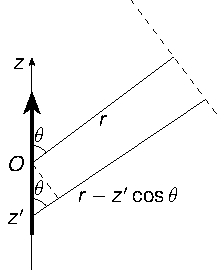
\includegraphics[width=0.9\textwidth]{Figures/Interference.pdf}
        \caption{Interference of electromagnetic waves}
        \label{fig:Interference}
    \end{figure}
\end{columns}
\end{frame}

\begin{frame}{Radiation pattern}
    \begin{columns}
        \column{0.5\textwidth}
            Fields of uniform line source
        \begin{align*}
            A_z &= \dfrac{ \exp ( -j \beta r) }{4 \pi r} \int_{-L/2}^{L/2} I(z') \exp( j \beta z') \mathrm{d}z' \\
            &= \dfrac{ \exp ( -j \beta r) }{4 \pi r} \dfrac{\sin [(\beta L/2) \cos (\theta)]}{(\beta L/2) \cos (\theta)}. \\
            \mathbf{E} &= j \omega \sin \theta A_z \mathbf{\hat{\theta}}.
        \end{align*}
        
        Radiation pattern:
        \begin{align*}
            &F(\theta,\phi) = \dfrac{E(\theta,\phi)}{E_{max}} = g(\theta) f(\theta,\phi) \\
            &= \sin \theta \cdot \dfrac{\sin [(\beta L/2) \cos (\theta)]}{(\beta L/2) \cos (\theta)}.
        \end{align*}
        \column{0.5\textwidth}
        \begin{figure}
            \centering
            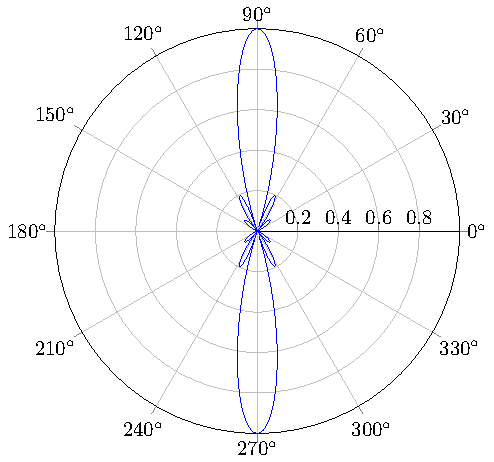
\includegraphics[width=\textwidth]{Figures/Radiation_pattern_diagram/Polar_plot.pdf}
            \caption{Radiation pattern with \( \beta L/2 = 10\).}
            \label{fig:Polar_radiation_pattern}
        \end{figure}
    \end{columns}
\end{frame}